\documentclass[11pt]{article}
\newcommand{\ReportDate}{28 October 2026}
% Preamble for the roughness technical report. Numbers are NOT typed here:
% they come from ../build/numbers.tex, generated by src/build_report.py.
\usepackage[T1]{fontenc}
\usepackage[utf8]{inputenc}
\usepackage{lmodern}
\usepackage[scaled=0.92]{helvet}
\usepackage[letterpaper,margin=1in,headheight=14pt]{geometry}
\usepackage{microtype}
\usepackage{amsmath}
\usepackage{graphicx}
\usepackage{booktabs,tabularx,array,makecell,longtable,threeparttable}
\usepackage[per-mode=symbol,detect-all]{siunitx}
\usepackage[table]{xcolor}
\usepackage[font=small,labelfont=bf,labelsep=period,justification=raggedright,singlelinecheck=false]{caption}
\usepackage{subcaption}
\usepackage{enumitem}
\usepackage{float}
\usepackage{placeins}
\usepackage{fancyhdr}
\usepackage[nobottomtitles*]{titlesec}
\renewcommand{\bottomtitlespace}{0.12\textheight}
\usepackage{textcomp}
\usepackage{tikz}
\usetikzlibrary{positioning,arrows.meta}
\usepackage[hidelinks]{hyperref}
\hypersetup{pdfauthor={Stephen Eacuello}}
\widowpenalty=10000 \clubpenalty=10000
\hyphenation{time-stamps}

\definecolor{ink}{HTML}{0B0B0B}
\definecolor{ink2}{HTML}{52514E}
\definecolor{rule}{HTML}{C9C8C2}
\definecolor{navy}{HTML}{002147}
\definecolor{note}{HTML}{F4F3EF}
\definecolor{gold}{HTML}{B8860B}

\sisetup{group-minimum-digits=5, round-mode=none}
\setlist{nosep, leftmargin=1.4em}
\setlength{\parskip}{0.45em}
\setlength{\parindent}{0pt}
\renewcommand{\arraystretch}{1.12}

\titleformat{\section}{\normalfont\sffamily\Large\bfseries\color{navy}}{\thesection}{0.6em}{}
\titleformat{\subsection}{\normalfont\sffamily\large\bfseries\color{navy}}{\thesubsection}{0.6em}{}
\titleformat{\subsubsection}{\normalfont\sffamily\normalsize\bfseries}{\thesubsubsection}{0.6em}{}
\titlespacing*{\section}{0pt}{1.2em}{0.5em}
\titlespacing*{\subsection}{0pt}{1.0em}{0.35em}

\pagestyle{fancy}
\fancyhf{}
\fancyhead[L]{\sffamily\footnotesize\color{ink2}Peak power of a small VAWT with textured blades}
\fancyhead[R]{\sffamily\footnotesize\color{ink2}\ReportDate}
\fancyfoot[C]{\sffamily\footnotesize\color{ink2}\thepage}
\renewcommand{\headrulewidth}{0.4pt}

% A shaded box for the bottom line.
\newsavebox{\keyboxbin}
\newenvironment{keybox}{\par\smallskip\noindent\begin{lrbox}{\keyboxbin}%
  \begin{minipage}{\dimexpr\linewidth-2\fboxsep-1.2pt\relax}}%
  {\end{minipage}\end{lrbox}\fcolorbox{rule}{note}{\usebox{\keyboxbin}}\par\smallskip}

\newcommand{\Ra}[1]{\ensuremath{\mathrm{Ra}\,#1}}
\newcommand{\pmax}{P_{\max}}
\newcommand{\figref}[1]{Fig.~\ref{#1}}
\newcommand{\tabref}[1]{Table~\ref{#1}}
\newcommand{\secref}[1]{Section~\ref{#1}}
\newcommand{\appref}[1]{Appendix~\ref{#1}}
% \input is not expandable, which breaks it between booktabs rules; @@input is.
\makeatletter\newcommand{\tabinput}[1]{\@@input #1 }\makeatother

\fancyhead[L]{\sffamily\footnotesize\color{ink2}CFD of the textured-blade turbine}
\hypersetup{pdftitle={CFD of the textured-blade turbine: summary of results},pdfauthor={Stephen Eacuello}}
\graphicspath{{./}}
\renewcommand{\topfraction}{0.9}\renewcommand{\bottomfraction}{0.8}
\renewcommand{\textfraction}{0.07}\renewcommand{\floatpagefraction}{0.8}
\renewcommand{\bottomtitlespace}{0.05\textheight}
\setcounter{topnumber}{3}\setcounter{bottomnumber}{2}\setcounter{totalnumber}{4}

\begin{document}
\thispagestyle{empty}
\begin{flushleft}
{\sffamily\small\color{ink2} SUMMARY \quad·\quad 28 OCTOBER 2026}\\[0.4em]
{\sffamily\LARGE\bfseries\color{navy} CFD of the textured-blade turbine}\\[0.3em]
{\sffamily\normalsize What 263 simulations show about blade roughness, and what to test next}\\[0.3em]
{\sffamily\small Stephen Eacuello \quad·\quad for Dr.\ Sodhi, Dr.\ Jahangiri and Dr.\ Jeong}
\end{flushleft}
{\color{rule}\hrule height 0.6pt}
\vspace{0.6em}

\begin{keybox}
\textbf{In short.} In the simulations, rough blades can increase the turbine's torque. The gain
comes mostly from the moment a blade moves edge-on into the wind, not from the cup-versus-back drag
that we expected to matter. With very rough blades (\SI{400}{\micro\metre}) the simulated torque rose
by about a third, the same direction as our wind-tunnel gains. With roughness closer to our printed
blades (\SI{100}{\micro\metre}) there was no clear change. The simulations are two-dimensional and
sensitive to their settings, so they cannot confirm the mechanism on their own: a direct force
measurement on a blade is the next step.
\end{keybox}

{\small\textit{A note on how this was done: I am not trained in aerodynamics or CFD. The simulations were set up, run and analyzed with the help of AI tools (Claude), which also helped draft this summary. Please treat the results as preliminary.}}

\section{Answers to the questions from our 7 October meeting}
{\small
\begin{longtable}{@{}>{\raggedright\arraybackslash}p{0.25\linewidth} >{\raggedright\arraybackslash}p{0.71\linewidth}@{}}
\toprule
Question & Answer \\
\midrule
\endfirsthead
\toprule
Question & Answer (continued) \\
\midrule
\endhead
\bottomrule
\endlastfoot
Lift and drag coefficients of the blade (theory and experiment) &
\textbf{From the CFD} (smooth blade, 23~m/s, 2D, chord \SI{48}{mm}):
cup facing the wind, drag 1.8--2.0 or about 3.2, depending on which of two flow patterns forms, with lift
near zero; edge-on, drag 0.35--0.42 and lift 0.7--1.1; back facing the wind, drag 1.5--1.7, falling to
1.1--1.2 with a finer time step. For comparison, published values for a thin half-tube are 2.3 (cup
facing) and 1.2 (back facing). \textbf{By experiment}: not yet measured; the force test is designed
(Section~\ref{sec:next}). \\
\addlinespace
A CFD model in OpenFOAM &
Done: 263 two-dimensional simulations of the blade and the rotor, summarised in the rest of this report. \\
\addlinespace
Cost and time per blade; a shorter blade? &
Print Lab slicer estimates, per blade: FS~0.10, 7~h~40~min, \SI{39}{g}, \$4.61; FS~0.20, 8~h~41~min,
\SI{41}{g}, \$5.15 (both with a \SI{0.2}{mm} nozzle); FS~0.80, 15~h~54~min, \SI{72}{g}, \$9.38 (with
a \SI{0.4}{mm} nozzle). The Print Lab charges \$0.50 per print hour plus material. A shorter blade
saves time and material roughly in proportion, but it changes the rotor, so it would need its own
Plain set for comparison. \\
\addlinespace
A rougher set (``\SI{320}{\micro\metre}'', \SI{0.805}{mm} fuzzy skin) &
The Print Lab has the print settings ready. We propose printing FS~0.40 and FS~0.80 together with a
fresh Plain set and repeats of FS~0.10 and FS~0.20, all with the same settings. ``Ra~320'' is a
label: FS~0.20 (``Ra~80'') measured Ra~\SI{10}{\micro\metre}, so we will scan the new blades. \\
\addlinespace
Is there a best roughness? &
Not known yet. In the CFD, very rough blades help the rotor, but realistic roughness gives no clear
change. The new print round (five levels, two prints each, tested in mixed order) is designed to find
it. \\
\addlinespace
What the Sandia report predicts for us &
Sandia (SAND2017-11288) tested lift-driven airfoils at much higher Reynolds numbers, where roughness
lowers lift and raises drag (4.9--6.8\,\% energy loss at \SI{200}{\micro\metre}). Our rotor is
drag-driven at low Reynolds numbers, where roughness can make the boundary layer turbulent earlier,
so Sandia does not predict a loss for us. Its roughness criterion suggests FS~0.20 reaches that point
at our higher wind speeds, and that rougher blades should start gaining at lower wind speeds and then
level off. The FS~0.40 and FS~0.80 tests can check this. \\
\end{longtable}
}

\section{Why we ran these simulations}
On 1 October, the FS~0.10 and FS~0.20 textured blades produced 12.8\,\% and 16.2\,\% more peak
electrical power than the Plain blades (averaged over 10.2--\SI{38}{m/s}). We used OpenFOAM to ask
two questions: how does roughness change the forces on a single blade, and how does it change the
torque of the whole rotor?

\section{What we simulated}
All runs are two-dimensional slices through the middle of the blade, at 23~m/s unless stated. They
ran on URI's Unity research computing cluster: 281 jobs and about 17{,}400 core-hours, using up to
512 processor cores at once. On a laptop this would have taken months.

\begin{table}[H]
\centering\small
\begin{tabularx}{\linewidth}{@{}l c X@{}}
\toprule
Model & Cases & What was varied \\
\midrule
Single blade & 194 & Angle to the wind (all the way round), wind speed (10.2, 23, \SI{38}{m/s}), roughness
height (smooth to \SI{400}{\micro\metre}), and the printed texture shape itself \\
Whole rotor (3 blades) & 69 & Tip-speed ratio (blade-tip speed divided by wind speed), wind speed,
roughness height, mesh resolution \\
\bottomrule
\end{tabularx}
\end{table}

\begin{figure}[tbp]
\centering
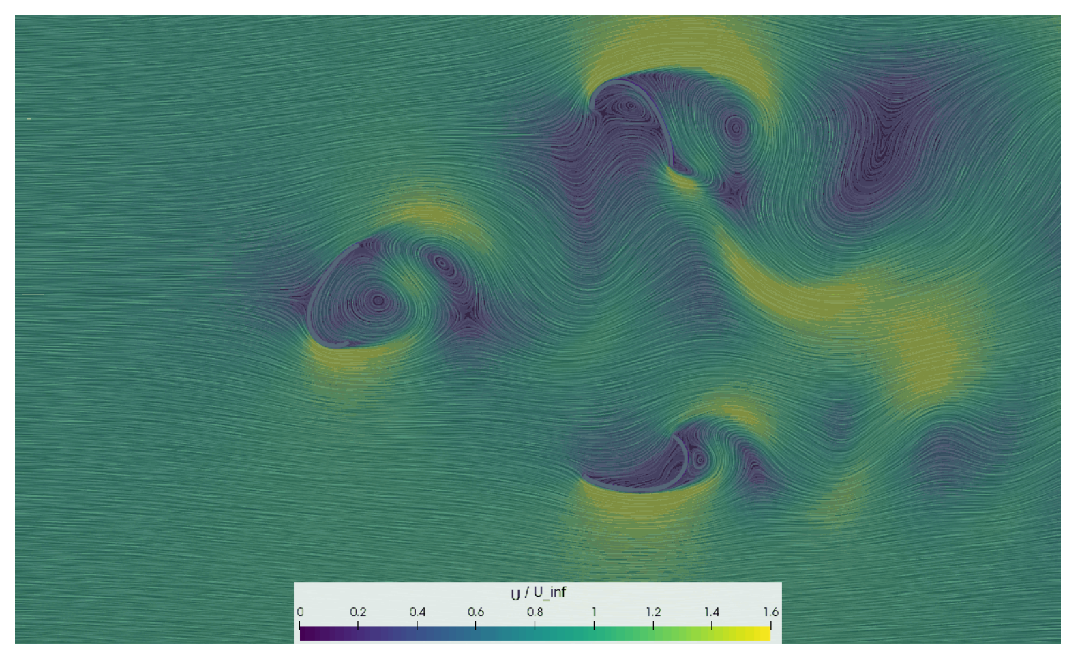
\includegraphics[width=0.85\linewidth]{fig4_rotor_flow}
\caption{A snapshot of the simulated rotor at 23~m/s, turning at 216~rpm (tip-speed ratio 0.10, rough
blades). The streaks follow the airflow; colour shows the local air speed relative to the oncoming wind
(yellow faster, dark slower). Each blade sheds swirls into the wake behind the rotor.}
\label{fig:rotorflow}
\end{figure}

Roughness enters the model as a uniform ``sand-grain'' height. Our blades' measured texture height
is about \SIrange{84}{97}{\micro\metre} for FS~0.20, so the \SI{100}{\micro\metre} cases are the
closest to the real blades; \SI{400}{\micro\metre} is a deliberately rough upper case.

\section{Results}

\subsection{On a single blade, roughness mostly changes the edge-on forces}
When the blade faces the wind cup-first or back-first, \SI{400}{\micro\metre} roughness changes the
drag by only about 6\,\%. When the blade is edge-on, the same roughness raises the drag by 45\,\% and
the lift by 67\,\% (Fig.~\ref{fig:blade}). At \SI{100}{\micro\metre} all changes are small (10\,\% or
less).

\begin{figure}[tbp]
\centering
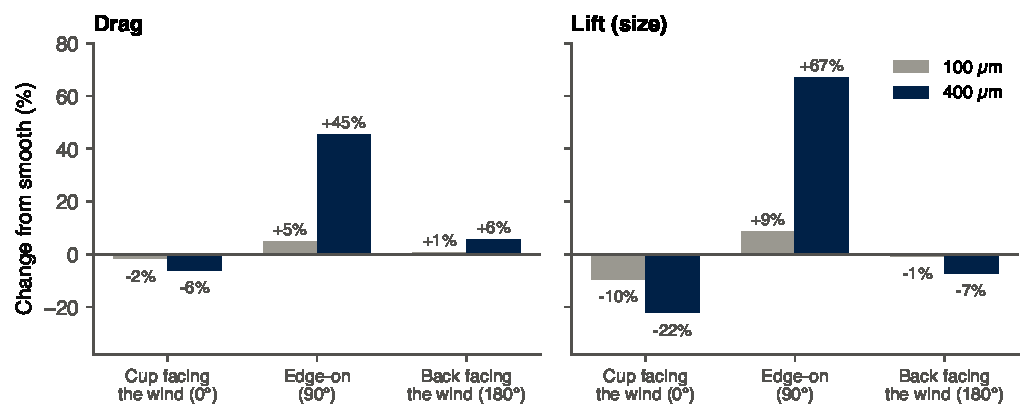
\includegraphics[width=0.95\linewidth]{fig1_single_blade}
\caption{Change in drag and lift on a single blade from roughness, compared with a smooth blade, for
three orientations (23~m/s).}
\label{fig:blade}
\end{figure}

\subsection{On the rotor, heavy roughness raises the torque}
With \SI{400}{\micro\metre} roughness, the rotor's torque rose by 27\,\% at a tip-speed ratio of 0.10
and by 38\,\% at 0.12 (Fig.~\ref{fig:rotor}). Our turbine reached peak power near a tip-speed ratio of
0.12--0.13 in the wind tunnel. At \SI{100}{\micro\metre} the changes (+8\,\% and $-19$\,\%) are within
the simulations' noise, so we cannot say whether realistic roughness helps or hurts in this model.

\begin{figure}[tbp]
\centering
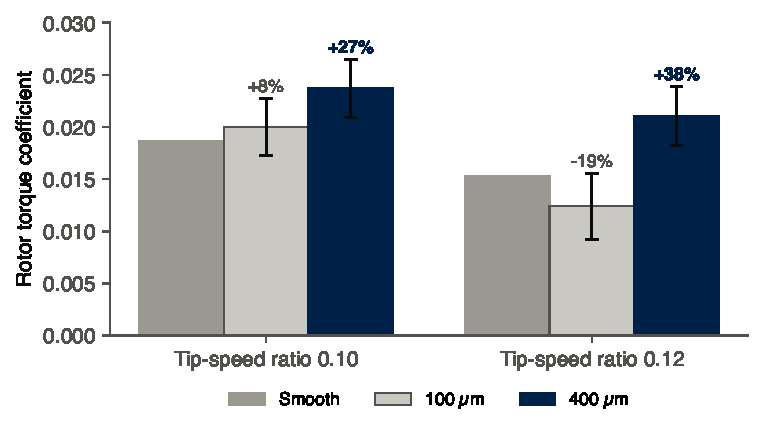
\includegraphics[width=0.72\linewidth]{fig2_rotor_torque}
\caption{Rotor torque with smooth and rough blades at two tip-speed ratios (23~m/s, averaged over 45
revolutions). Error bars show the simulations' noise; a change is clear when it is larger than the
bar.}
\label{fig:rotor}
\end{figure}

\subsection{The gain comes from the blade moving edge-on with the wind}
Splitting the turn into positions shows where the extra torque comes from (Fig.~\ref{fig:where}). The
blade moving edge-on with the wind contributes the most (+49\,\% of the smooth rotor's torque). Some
is lost when the blade moves edge-on against the wind ($-26$\,\%). This matches the single-blade
result: the edge-on forces are the ones roughness changes most. Our earlier, simpler estimate (13
October) looked only at the cup-facing and back-facing positions, which is why it predicted a loss.

\begin{figure}[tbp]
\centering
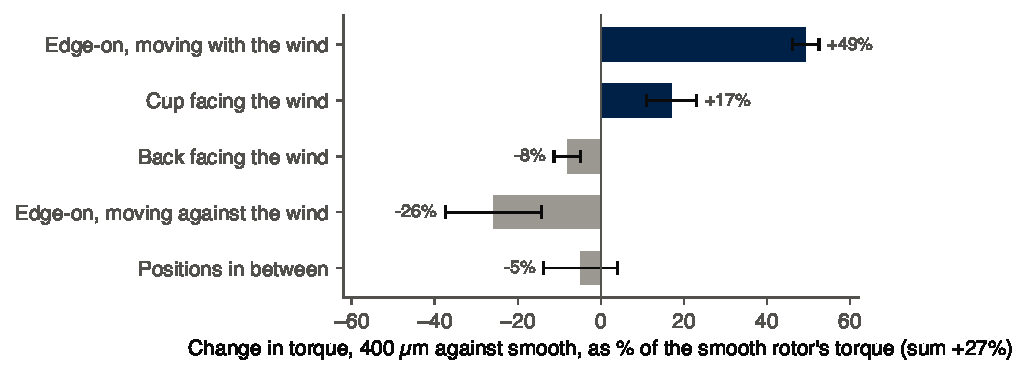
\includegraphics[width=0.8\linewidth]{fig3_where_in_the_turn}
\caption{Where in each turn the \SI{400}{\micro\metre} blades gain or lose torque, as a percentage of
the smooth rotor's torque (tip-speed ratio 0.10). The parts add up to the +27\,\% of
Fig.~\ref{fig:rotor}.}
\label{fig:where}
\end{figure}

\section{How much to trust this}
\begin{itemize}
\item \textbf{The simulations are two-dimensional.} Flow around a curved blade is three-dimensional,
  and 2D simulations of this kind usually overstate drag. The results are best read as comparisons
  between cases rather than as absolute values.
\item \textbf{The rotor result is promising but not yet firm.} The rotor's torque changes more between
  mesh resolutions than it does with roughness. We assumed that this affects smooth and rough runs
  the same way, but have not shown it.
\item \textbf{The model's roughness is not our texture.} The printed fuzzy skin is not a uniform sand-grain
  surface, and we do not yet know which roughness height represents it.
\item \textbf{One flow pattern is uncertain.} With the cup facing the wind, the simulated flow can settle
  into either of two stable patterns, one with nearly twice the drag of the other. Only a measurement can
  tell which one the real blade has (Fig.~\ref{fig:patterns}).
\end{itemize}

\begin{figure}[tbp]
\centering
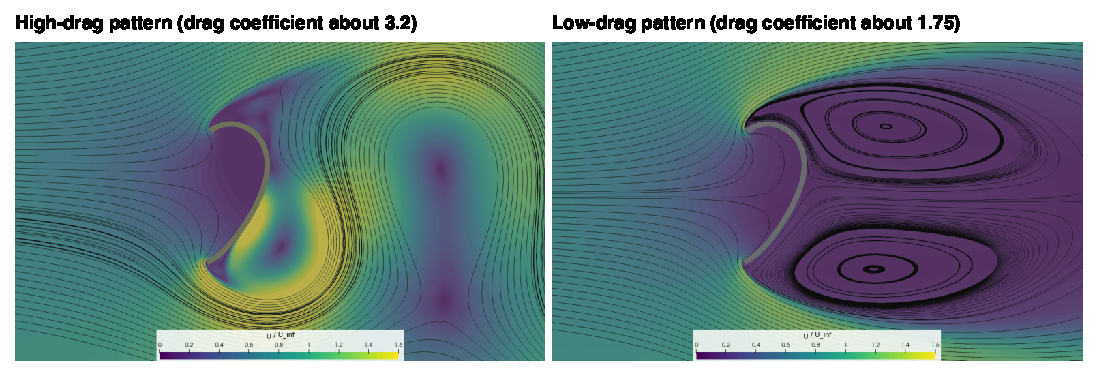
\includegraphics[width=\linewidth]{fig5_two_flow_patterns}
\caption{The two flow patterns the simulation can settle into with the cup facing the wind (smooth
blade, 23~m/s). Left: the wake swings from side to side and sheds large swirls. Right: two steady
swirls sit behind the cup. The blade and mesh are the same; only the simulation's time step differs.}
\label{fig:patterns}
\end{figure}

\section{Proposed next steps}\label{sec:next}
\begin{enumerate}
\item \textbf{Measure lift and drag on single blades} (the ``airfoil slice'' test). An existing Plain
  blade and a textured blade, half in the wind, on a small two-load-cell balance under the tunnel
  floor, at the cup-facing, edge-on and back-facing angles. This tests the main simulation result
  directly. The design is ready; parts cost about \$250--450.
\item \textbf{Test rougher blades.} Print FS~0.40 and FS~0.80 (the ``\SI{320}{\micro\metre}'' set)
  together with a fresh Plain set and repeats of FS~0.10 and FS~0.20, all with the same print
  settings, and test them in one session. I will ask the Print Lab for time and cost estimates.
\item \textbf{Record the rig details} the simulations had to assume: how the blades attach to the arms,
  which way the rotor turns, and the tunnel's test-section size.
\end{enumerate}
Since the MCE labs now also use the tunnel, I am coordinating test times with Jim Byrnes and Rob
D'Ambrosca.

\vspace{0.6em}
{\small\color{ink2}Details, all figures and the scripts behind every number:
\texttt{cfd/analysis/2026-10-15/} in the project repository.}

\end{document}
